\chapter{Lecture 32 - Solving Non-linear BVPs with Finite Difference Methods}
\label{ch:lec32n}
\section{Objectives}
The objectives of this lecture are to:
\begin{itemize}
\item Describe a way to solve non-linear BVPs with Finite Difference Methods.
\item Illustrate the method through an example.
\end{itemize}
\setcounter{lstannotation}{0}

\section{A Non-Linear Boundary Value Problem}
We will use the Finite Difference Method to solve the same problem that we tackled in Lecture 28.  At risk of offending readers through gratuitous repetition, we will recall the problem statement here.

\vspace{0.25cm}

\noindent\textbf{Problem Statement:}

\vspace{0.1cm}

\noindent A pin fin is a slender extension attached to increase the surface area and enable greater heat transfer.  When convection and radiation are included in the analysis, the steady-state temperature distribution, $T(x)$, along a pin fin can be caluclated from the solution of the equation below:
\begin{equation}
\frac{d^2T}{dx^2} - \frac{h_cP}{kA_c}\left(T - T_s\right)-\frac{\epsilon \sigma_{SB}P}{k A_c}\left(T^4 - T_s^4 \right) = 0, \ \ 0 \le x \le 0.1
\end{equation}
with boundary conditions $T(0)=T_A$ and $T(0.1)=T_B$.  A schematic of the system is shown in Figure \ref{fig:lec31n-ex1-schematic}.  There are a number of parameters given in the equation.  These are specified in Table \ref{tab:lec31n-ex1-parameters}.
\begin{marginfigure}[-4.5cm]
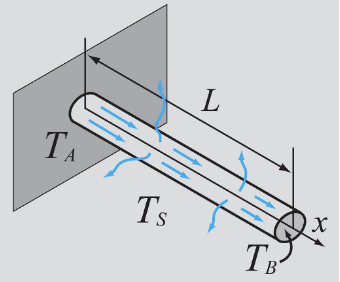
\includegraphics{lec28n-ex1-schematic.png}
\caption{Pin Fin Boundary Value Problem Schematic.}
\label{fig:lec31n-ex1-schematic}
\end{marginfigure}

\begin{table}
\begin{tabular}{|c|c|}
\hline
\textbf{Parameter} & \textbf{Value} \\ \hline
Convective heat transfer coefficient ($h_c$) & 40 $\text{W}/\text{m}^2\text{-K}$ \\ \hline
Perimeter of the pin ($P$) & 0.016 m \\ \hline
Radiative emissivity of the surface ($\epsilon$) & 0.4 \\ \hline
Thermal conductivity of the pin material ($k$) & 240 $\text{W}/\text{m-K}$ \\ \hline
Cross-sectional area of the fin ($A_c$) & $1.6 \times 10^{-5} \text{m}^2$ \\ \hline
Temperature of surrounding air ($T_S$) & 293 K \\ \hline
Stefan-Boltzmann constant ($\sigma_{SB}$) & $5.67 \times 10^{-8} \text{W}/\text{m}^2\text{-K}^4$ \\ \hline
Temperature of fin at base ($T_A$) & 473 K \\ \hline
Temperature of fin at end ($T_B$) & 293 K \\ \hline
\end{tabular}
\caption{Example problem parameters.}
\label{tab:lec31n-ex1-parameters}
\end{table}

\newthought{We want to} use the FDM which, as we saw last lecture, usually involves replacing the differential operators with their discrete finite difference equivalent.  We then form a linear system of equations and solve it.  The problem here is that the system of equations that we obtain is \emph{non-linear}.  The reason for this non-linearity is, as readers should know, the term involving $T^4$.\marginnote{\textbf{Reminder:} A differential equation is \emph{non-linear} when the \emph{dependent variable} or any of its derivatives appear in a non-linear term in the governing equation. }

We will address this problem with the following method:

\begin{enumerate}
\item \textbf{Step \#1:} Re-arrange the equation to put non-homogeneous and non-linear terms on the right-hand side.  

\vspace{0.25cm}

\noindent Carrying out this task for the governing equation for our example problem gives us:

\begin{equation*}
\frac{d^2 T}{dx^2} - \underbrace{\frac{h_c P}{k A_{c}}}_{\alpha_1}T = \underbrace{\frac{h_c P}{k A_c}}_{\alpha_1} T_s + \underbrace{\frac{\epsilon \sigma_{SB}}{kA_c}}_{\alpha_2}\left(T^4 - T_s^4 \right)
\end{equation*}

\item \textbf{Step \#2:} Apply finite difference approximations to linear terms and apply boundary conditions.

\marginnote{
\vspace{1.5cm}

\noindent Note that the term $b$ on the right-hand side is constant.  The term $\phi(T)$ is the non-linear term in the dependent variable.  $L$ is the linear operator with appropriate modifications to incorporate the Dirichlet boundary conditions.
}
\begin{align*}
\text{Dxx}T - \alpha_1 \left[I\right] T &= \alpha_1 \left[I\right]T_s + \alpha_2 \left[I\right]\left(T^4-T_s\right) \\
\underbrace{\left(\text{D}_{xx} - \alpha_1\left[I\right]\right)}_{L}T &= \underbrace{\left(\alpha_1 \left[I\right]T_s - \alpha_2 \left[I\right]T_s^4\right)}_{b} + \alpha_2\left[I\right]T^4 \\
LT &= b - \underbrace{\alpha_2 \left[I\right]T^4}_{\phi(T)}
\end{align*}

\item \textbf{Step \#3:} Apply current (or initial) value of dependent variable to the non-linear term, $\phi(T)$. \marginnote{
\vspace{0.1cm}

\noindent\textbf{Note:} Elements of $T$ corresponding to boundaries are maintained constant and equal to the specified boundary conditions.
}

\begin{equation*}
LT = b - \phi(T_i)
\end{equation*}

\item \textbf{Step \#4:} Solve the lineary system of equations and evaluate the relative change in the dependent variable.

\begin{align*}
T_{i+1} &= L^{-1} \left[b - \phi(T_i)\right] \\
\epsilon &= \frac{||T_{i+1} - T_i||}{||T_i||}
\end{align*}

\item Repeate Steps \#3 and \#4 until $\epsilon < \text{TOL}$ for some specified tolerance.

\end{enumerate}
This is a form of \emph{fixed point iteration}. Looking again at the equation in Step \#4 above:
\begin{equation*}
T_{i+1} = L^{-1}\left[b-\phi(T_{i})\right] = g(T_i)
\end{equation*}
The solution we are looking for is when $g(T_i) \rightarrow T_i$; this is called a \emph{fixed point}.  The conditions under which $g(T)$ will \emph{have} a fixed point are beyond the scope of this class and will not be discussed further in this lecture.\sidenote{Interested readers can learn more about the Banach fixed point theorm which says, roughly, that if $g(T)$ is a \emph{contraction mapping} (at least in some region ``close'' to a fixed point) then the fixed point iteration will succeed. This is, suffice it to say, a loose statement.}

\section{MATLAB Implementation}
A listing of MATLAB code that implements the method described above for our example problem is provided below.

\noindent We begin by clearing the workspace and defining constants.
\begin{lstlisting}[style=myMatlab,name=lec32n-ex]
clear
clc
close 'all'

%% Define constants
a = 0; b = 0.1;
N = 2000;
Ac = 1.6e-5; % m^2, fin cross sectional area
P = 0.016; % m, perimeter of pin cross section
h_c = 40; % W/m^2-K, convective heat transfer coefficient 
k = 250; % W/m-K, thermal conductivity of pin material
emiss = 0.5; % emissivity of pin material
sigma_sb = 5.67e-8; % W/m^2-K^4, Stefan-Boltzmann constant
Ts = 293; % K, temperature of surrounding air

% Boundary Conditions
Ta = 473;  Tb = 293;
\end{lstlisting}


\noindent Next we construct the differential operators and apply boundary conditions to them.
\begin{lstlisting}[style=myMatlab,name=lec32n-ex]
% Discretize the space and get Operators
x = linspace(a,b,N); x = x';

Dx_op = Dx(a,b,N);
Dxx_op = Dxx(a,b,N);
alpha_1 = h_c*P/(k*Ac);
alpha_2 = emiss*sigma_sb*P/(k*Ac);
L = Dxx_op - alpha_1*speye(N,N);

% apply boundary condition to L
L(1,:) = 0; L(1,1) = 1; 
L(N,:) = 0; L(N,N) = 1;

\end{lstlisting}

In order to form the right-hand side of our system of equations, we need to estimate the temperature distribution.  It's probably not fair since we have solved this problem before but, given the boundary conditions, a linear initial guess between the fin root and tip makes a lot of sense.

\begin{lstlisting}[style=myMatlab,name=lec32n-ex]
% Estimate initial temperature distribution
To = linspace(Ta,Tb,N); To = To';

% Form RHS
b = -ones(N,1)*Ts*alpha_1 - ones(N,1)*(Ts^4)*alpha_2;
phi = (To.^4)*alpha_2;
RHS = b - phi;

% apply BC to RHS
RHS(1) = Ta; RHS(N) = Tb;

\end{lstlisting}

Now we are ready to apply the fixed-point iteration scheme.
\begin{lstlisting}[style=myMatlab,name=lec32n-ex]
tol = 1e-7; imax = 100; T = To;

for i = 1:imax

    %solve the system of equations for new estimate of temperature
    Tnew = L\RHS;     
    % obtain convergence criterion "error estimate"
    Err = norm(T - Tnew,Inf)/norm(T,Inf);    
    % exit loop if error is within tolerance
    if Err <tol
        fprintf('Success!! Iteration converged after %d iterations.\n',i);
        fprintf('Error estimate: %g \n',Err);
        break;
    end    
    % error tolerance not met, prepare for next iteration
    phi = (Tnew.^4)*alpha_2;
    RHS = b - phi;
    RHS(1) = Ta; RHS(N) = Tb; %re-apply BC   
    T = Tnew;
    
end

if i == imax
    fprintf('Error! Solution not converged after %i iterations.\n',imax);
    fprintf('Last residual = %g \n',Err);
end

fprintf('\n\n Plotting Last Solution: \n\n');
figure(1)
plot(x,T,'-r','linewidth',3);
title('Solution of Non-linear BVP with Finite Difference Method',...
    'fontsize',16,'fontweight','bold');
xlabel('X (m) ','fontsize',14,'fontweight','bold');
ylabel('T (K) ','fontsize',14,'fontweight','bold');
set(gca,'fontsize',12,'fontweight','bold');
grid on
\end{lstlisting}
\begin{marginfigure}
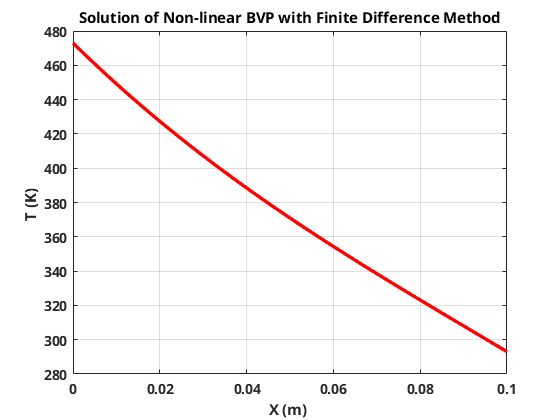
\includegraphics{lec32n-ex-sol.png}
\caption{Solution of example problem with Finite Difference Methods}
\label{fig:lec32n-ex-sol}
\end{marginfigure}
The temperature distribution obtained using this method is shown in Figure \ref{fig:lec32n-ex-sol}.  The result required 5 iterations with a relative error of $5.8\times 10^{-9}$.
